% CSBP441 Phase 2 final report - CVPR author kit (tools/cvpr_kit, CVPR2027-v1), camera-ready mode
\documentclass[10pt,twocolumn,letterpaper]{article}
\usepackage[pagenumbers]{cvpr}

% tectonic is XeTeX: the Type-1 `times` package has no TU encoding, so load the Times/Helvetica/Courier clones
\usepackage{fontspec}
\setmainfont{texgyretermes}[Extension=.otf,UprightFont=*-regular,BoldFont=*-bold,ItalicFont=*-italic,BoldItalicFont=*-bolditalic]
\setsansfont{texgyreheros}[Extension=.otf,UprightFont=*-regular,BoldFont=*-bold,ItalicFont=*-italic,BoldItalicFont=*-bolditalic]
\setmonofont{texgyrecursor}[Extension=.otf,UprightFont=*-regular,BoldFont=*-bold,ItalicFont=*-italic,BoldItalicFont=*-bolditalic]
\usepackage{multirow}
\usepackage{microtype}
\setlength{\abovecaptionskip}{3pt}
\setlength{\textfloatsep}{8pt plus 2pt minus 2pt}
\setlength{\floatsep}{6pt plus 2pt minus 2pt}
\setlength{\dbltextfloatsep}{8pt plus 2pt minus 2pt}
\definecolor{cvprblue}{rgb}{0.21,0.49,0.74}
\usepackage[breaklinks,colorlinks,allcolors=cvprblue]{hyperref}

% generated by scripts/latex_tables.py from results/*.csv - do not edit
\newcommand{\faceFARnormal}{0.94}
\newcommand{\faceFRRnormal}{0.2}
\newcommand{\latArcmediapipe}{10.0}
\newcommand{\latExtramediapipe}{+6.4}
\newcommand{\latPmediapipeFull}{22.2}
\newcommand{\latPmediapipeRoi}{28.7}
\newcommand{\latmediapipeFull}{15.6}
\newcommand{\latmediapipeRoi}{22.1}
\newcommand{\lfwTestAcc}{98.9}
\newcommand{\lfwTestFAR}{0.4}
\newcommand{\lfwTestFRR}{1.8}
\newcommand{\lfwThr}{0.2235}
\newcommand{\mpAccFarSFiveUp}{64.2}
\newcommand{\mpAccFarSFiveUpScrfd}{90.6}
\newcommand{\mpAccFarSFourUp}{64.4}
\newcommand{\mpAccFarSFourUpScrfd}{72.6}
\newcommand{\mpAccFarSSixUp}{64.2}
\newcommand{\mpAccFarSSixUpScrfd}{94.0}
\newcommand{\mpAccFarSThreeNoup}{64.8}
\newcommand{\mpAccFarSThreeUp}{64.6}
\newcommand{\mpAccFarSThreeUpScrfd}{29.4}
\newcommand{\mpAccFarSThreeUpyZeroFive}{64.6}
\newcommand{\mpAccFarSTwoUp}{63.2}
\newcommand{\mpAccFarSTwoUpScrfd}{3.0}
\newcommand{\mpAccFarfull}{63.6}
\newcommand{\mpAccSFiveUp}{74.6}
\newcommand{\mpAccSFiveUpScrfd}{83.1}
\newcommand{\mpAccSFourUp}{73.1}
\newcommand{\mpAccSFourUpScrfd}{66.0}
\newcommand{\mpAccSSixUp}{74.6}
\newcommand{\mpAccSSixUpScrfd}{85.5}
\newcommand{\mpAccSThreeNoup}{62.8}
\newcommand{\mpAccSThreeUp}{61.6}
\newcommand{\mpAccSThreeUpScrfd}{26.1}
\newcommand{\mpAccSThreeUpyZeroFive}{62.2}
\newcommand{\mpAccSTwoUp}{41.1}
\newcommand{\mpAccSTwoUpScrfd}{2.5}
\newcommand{\mpAccfull}{72.9}
\newcommand{\mpBaseAllAcc}{72.9}
\newcommand{\mpBaseCroAcc}{70.0}
\newcommand{\mpBaseFarAcc}{63.6}
\newcommand{\mpBaseLowAcc}{67.0}
\newcommand{\mpBaseNorAcc}{91.0}
\newcommand{\mpBgSFiveUp}{16.2}
\newcommand{\mpBgSFiveUpScrfd}{16.2}
\newcommand{\mpBgSFourUp}{15.2}
\newcommand{\mpBgSFourUpScrfd}{12.9}
\newcommand{\mpBgSSixUp}{17.4}
\newcommand{\mpBgSSixUpScrfd}{17.7}
\newcommand{\mpBgSThreeNoup}{15.7}
\newcommand{\mpBgSThreeUp}{15.4}
\newcommand{\mpBgSThreeUpScrfd}{5.1}
\newcommand{\mpBgSThreeUpyZeroFive}{15.9}
\newcommand{\mpBgSTwoUp}{15.4}
\newcommand{\mpBgSTwoUpScrfd}{1.0}
\newcommand{\mpBgfull}{22.0}
\newcommand{\mpBiasFullagegroupMid}{72.1}
\newcommand{\mpBiasFullagegroupOld}{68.7}
\newcommand{\mpBiasFullagegroupYoung}{78.1}
\newcommand{\mpBiasFullgenderfemale}{73.0}
\newcommand{\mpBiasFullgendermale}{72.8}
\newcommand{\mpBiasFullraceAsian}{72.5}
\newcommand{\mpBiasFullraceBlack}{75.5}
\newcommand{\mpBiasFullraceIndian}{95.0}
\newcommand{\mpBiasFullraceWhite}{72.3}
\newcommand{\mpBiasNagegroupMid}{38}
\newcommand{\mpBiasNagegroupOld}{31}
\newcommand{\mpBiasNagegroupYoung}{31}
\newcommand{\mpBiasNgenderfemale}{62}
\newcommand{\mpBiasNgendermale}{38}
\newcommand{\mpBiasNraceAsian}{4}
\newcommand{\mpBiasNraceBlack}{11}
\newcommand{\mpBiasNraceIndian}{1}
\newcommand{\mpBiasNraceWhite}{84}
\newcommand{\mpBiasTagegroupMid}{84.2}
\newcommand{\mpBiasTagegroupOld}{84.4}
\newcommand{\mpBiasTagegroupYoung}{88.4}
\newcommand{\mpBiasTgenderfemale}{85.6}
\newcommand{\mpBiasTgendermale}{85.4}
\newcommand{\mpBiasThreeagegroupMid}{59.2}
\newcommand{\mpBiasThreeagegroupOld}{59.0}
\newcommand{\mpBiasThreeagegroupYoung}{67.1}
\newcommand{\mpBiasThreegenderfemale}{62.0}
\newcommand{\mpBiasThreegendermale}{60.9}
\newcommand{\mpBiasThreeraceAsian}{71.2}
\newcommand{\mpBiasThreeraceBlack}{57.7}
\newcommand{\mpBiasThreeraceIndian}{55.0}
\newcommand{\mpBiasThreeraceWhite}{61.7}
\newcommand{\mpBiasTraceAsian}{81.2}
\newcommand{\mpBiasTraceBlack}{85.0}
\newcommand{\mpBiasTraceIndian}{95.0}
\newcommand{\mpBiasTraceWhite}{85.7}
\newcommand{\mpFARbgFull}{13.6}
\newcommand{\mpFARbgRoiSix}{0.8}
\newcommand{\mpFARbgRoiThree}{7.1}
\newcommand{\mpFRRFull}{30.1}
\newcommand{\mpFRRFullcrowded}{36.8}
\newcommand{\mpFRRFullfar}{36.4}
\newcommand{\mpFRRFulllowlight}{33.4}
\newcommand{\mpFRRFullnormal}{9.8}
\newcommand{\mpFRRRoiSix}{15.3}
\newcommand{\mpFRRRoiSixcrowded}{22.6}
\newcommand{\mpFRRRoiSixfar}{6.6}
\newcommand{\mpFRRRoiSixlowlight}{23.6}
\newcommand{\mpFRRRoiSixnormal}{6.5}
\newcommand{\mpFRRRoiThree}{40.4}
\newcommand{\mpFRRRoiThreecrowded}{39.2}
\newcommand{\mpFRRRoiThreefar}{35.6}
\newcommand{\mpFRRRoiThreelowlight}{53.2}
\newcommand{\mpFRRRoiThreenormal}{31.8}
\newcommand{\mpFaceSFiveUp}{50.3}
\newcommand{\mpFaceSFiveUpScrfd}{99.2}
\newcommand{\mpFaceSFiveUpScrfdcrowded}{100.0}
\newcommand{\mpFaceSFiveUpScrfdfar}{99.0}
\newcommand{\mpFaceSFiveUpScrfdlowlight}{98.2}
\newcommand{\mpFaceSFiveUpScrfdnormal}{99.7}
\newcommand{\mpFaceSFiveUpcrowded}{52.8}
\newcommand{\mpFaceSFiveUpfar}{13.7}
\newcommand{\mpFaceSFiveUplowlight}{63.7}
\newcommand{\mpFaceSFiveUpnormal}{71.2}
\newcommand{\mpFaceSFourUp}{50.3}
\newcommand{\mpFaceSFourUpScrfd}{99.2}
\newcommand{\mpFaceSFourUpScrfdcrowded}{100.0}
\newcommand{\mpFaceSFourUpScrfdfar}{99.0}
\newcommand{\mpFaceSFourUpScrfdlowlight}{98.2}
\newcommand{\mpFaceSFourUpScrfdnormal}{99.7}
\newcommand{\mpFaceSFourUpcrowded}{52.8}
\newcommand{\mpFaceSFourUpfar}{13.7}
\newcommand{\mpFaceSFourUplowlight}{63.7}
\newcommand{\mpFaceSFourUpnormal}{71.2}
\newcommand{\mpFaceSSixUp}{50.3}
\newcommand{\mpFaceSSixUpScrfd}{99.2}
\newcommand{\mpFaceSSixUpScrfdcrowded}{100.0}
\newcommand{\mpFaceSSixUpScrfdfar}{99.0}
\newcommand{\mpFaceSSixUpScrfdlowlight}{98.2}
\newcommand{\mpFaceSSixUpScrfdnormal}{99.7}
\newcommand{\mpFaceSSixUpcrowded}{52.8}
\newcommand{\mpFaceSSixUpfar}{13.7}
\newcommand{\mpFaceSSixUplowlight}{63.7}
\newcommand{\mpFaceSSixUpnormal}{71.2}
\newcommand{\mpFaceSThreeNoup}{50.3}
\newcommand{\mpFaceSThreeNoupcrowded}{52.8}
\newcommand{\mpFaceSThreeNoupfar}{13.7}
\newcommand{\mpFaceSThreeNouplowlight}{63.7}
\newcommand{\mpFaceSThreeNoupnormal}{71.2}
\newcommand{\mpFaceSThreeUp}{50.3}
\newcommand{\mpFaceSThreeUpScrfd}{99.2}
\newcommand{\mpFaceSThreeUpScrfdcrowded}{100.0}
\newcommand{\mpFaceSThreeUpScrfdfar}{99.0}
\newcommand{\mpFaceSThreeUpScrfdlowlight}{98.2}
\newcommand{\mpFaceSThreeUpScrfdnormal}{99.7}
\newcommand{\mpFaceSThreeUpcrowded}{52.8}
\newcommand{\mpFaceSThreeUpfar}{13.7}
\newcommand{\mpFaceSThreeUplowlight}{63.7}
\newcommand{\mpFaceSThreeUpnormal}{71.2}
\newcommand{\mpFaceSThreeUpyZeroFive}{50.3}
\newcommand{\mpFaceSThreeUpyZeroFivecrowded}{52.8}
\newcommand{\mpFaceSThreeUpyZeroFivefar}{13.7}
\newcommand{\mpFaceSThreeUpyZeroFivelowlight}{63.7}
\newcommand{\mpFaceSThreeUpyZeroFivenormal}{71.2}
\newcommand{\mpFaceSTwoUp}{50.3}
\newcommand{\mpFaceSTwoUpScrfd}{99.2}
\newcommand{\mpFaceSTwoUpScrfdcrowded}{100.0}
\newcommand{\mpFaceSTwoUpScrfdfar}{99.0}
\newcommand{\mpFaceSTwoUpScrfdlowlight}{98.2}
\newcommand{\mpFaceSTwoUpScrfdnormal}{99.7}
\newcommand{\mpFaceSTwoUpcrowded}{52.8}
\newcommand{\mpFaceSTwoUpfar}{13.7}
\newcommand{\mpFaceSTwoUplowlight}{63.7}
\newcommand{\mpFaceSTwoUpnormal}{71.2}
\newcommand{\mpSAllAcc}{61.6}
\newcommand{\mpSAllBrk}{283}
\newcommand{\mpSAllD}{$-$11.3}
\newcommand{\mpSAllFix}{57}
\newcommand{\mpSAllHi}{$-$9.6}
\newcommand{\mpSAllLo}{$-$13.1}
\newcommand{\mpSAllP}{<0.001}
\newcommand{\mpSAnchor}{BlazeFace}
\newcommand{\mpSCroAcc}{66.8}
\newcommand{\mpSCroBrk}{45}
\newcommand{\mpSCroD}{$-$3.2}
\newcommand{\mpSCroFix}{29}
\newcommand{\mpSCroHi}{+0.2}
\newcommand{\mpSCroLo}{$-$6.8}
\newcommand{\mpSCroP}{0.081}
\newcommand{\mpSErrBaselineAlsoWrong}{485}
\newcommand{\mpSErrErrors}{768}
\newcommand{\mpSErrErrorsCrowded}{166}
\newcommand{\mpSErrErrorsFar}{177}
\newcommand{\mpSErrErrorsLowLight}{264}
\newcommand{\mpSErrErrorsNormal}{161}
\newcommand{\mpSErrNoDetectionInRoi}{356}
\newcommand{\mpSErrNoFaceFound}{380}
\newcommand{\mpSErrWrongClass}{32}
\newcommand{\mpSFarAcc}{64.6}
\newcommand{\mpSFarBrk}{6}
\newcommand{\mpSFarD}{+1.0}
\newcommand{\mpSFarFix}{11}
\newcommand{\mpSFarHi}{+2.6}
\newcommand{\mpSFarLo}{$-$0.6}
\newcommand{\mpSFarP}{0.33}
\newcommand{\mpSLowAcc}{47.2}
\newcommand{\mpSLowBrk}{113}
\newcommand{\mpSLowD}{$-$19.8}
\newcommand{\mpSLowFix}{14}
\newcommand{\mpSLowHi}{$-$15.8}
\newcommand{\mpSLowLo}{$-$23.6}
\newcommand{\mpSLowP}{<0.001}
\newcommand{\mpSNorAcc}{67.8}
\newcommand{\mpSNorBrk}{119}
\newcommand{\mpSNorD}{$-$23.2}
\newcommand{\mpSNorFix}{3}
\newcommand{\mpSNorHi}{$-$19.6}
\newcommand{\mpSNorLo}{$-$27.0}
\newcommand{\mpSNorP}{<0.001}
\newcommand{\mpSScale}{3}
\newcommand{\mpTAllAcc}{85.5}
\newcommand{\mpTAllBrk}{73}
\newcommand{\mpTAllD}{+12.7}
\newcommand{\mpTAllFix}{326}
\newcommand{\mpTAllHi}{+14.5}
\newcommand{\mpTAllLo}{+10.7}
\newcommand{\mpTAllP}{<0.001}
\newcommand{\mpTAnchor}{SCRFD}
\newcommand{\mpTCroAcc}{77.4}
\newcommand{\mpTCroBrk}{39}
\newcommand{\mpTCroD}{+7.4}
\newcommand{\mpTCroFix}{76}
\newcommand{\mpTCroHi}{+11.4}
\newcommand{\mpTCroLo}{+3.4}
\newcommand{\mpTCroP}{<0.001}
\newcommand{\mpTErrBaselineAlsoWrong}{216}
\newcommand{\mpTErrErrors}{289}
\newcommand{\mpTErrErrorsCrowded}{113}
\newcommand{\mpTErrErrorsFar}{30}
\newcommand{\mpTErrErrorsLowLight}{115}
\newcommand{\mpTErrErrorsNormal}{31}
\newcommand{\mpTErrNoDetectionInRoi}{189}
\newcommand{\mpTErrNoFaceFound}{16}
\newcommand{\mpTErrWrongClass}{84}
\newcommand{\mpTFarAcc}{94.0}
\newcommand{\mpTFarBrk}{6}
\newcommand{\mpTFarD}{+30.4}
\newcommand{\mpTFarFix}{158}
\newcommand{\mpTFarHi}{+34.6}
\newcommand{\mpTFarLo}{+26.2}
\newcommand{\mpTFarP}{<0.001}
\newcommand{\mpTLowAcc}{77.0}
\newcommand{\mpTLowBrk}{22}
\newcommand{\mpTLowD}{+10.0}
\newcommand{\mpTLowFix}{72}
\newcommand{\mpTLowHi}{+14.0}
\newcommand{\mpTLowLo}{+6.4}
\newcommand{\mpTLowP}{<0.001}
\newcommand{\mpTNorAcc}{93.8}
\newcommand{\mpTNorBrk}{6}
\newcommand{\mpTNorD}{+2.8}
\newcommand{\mpTNorFix}{20}
\newcommand{\mpTNorHi}{+4.8}
\newcommand{\mpTNorLo}{+1.0}
\newcommand{\mpTNorP}{0.0094}
\newcommand{\mpTScale}{6}
\newcommand{\mpValSFive}{71.8}
\newcommand{\mpValSFivescrfd}{78.3}
\newcommand{\mpValSFour}{69.7}
\newcommand{\mpValSFourscrfd}{65.0}
\newcommand{\mpValSSix}{70.7}
\newcommand{\mpValSSixscrfd}{81.4}
\newcommand{\mpValSThree}{58.9}
\newcommand{\mpValSThreescrfd}{31.4}
\newcommand{\mpValSTwo}{35.7}
\newcommand{\mpValSTwoscrfd}{4.4}
\newcommand{\mpValfull}{69.6}
\newcommand{\mpWrongAnchorSFiveUp}{10.4}
\newcommand{\mpWrongAnchorSFiveUpScrfd}{17.5}
\newcommand{\mpWrongAnchorSFourUp}{10.4}
\newcommand{\mpWrongAnchorSFourUpScrfd}{17.5}
\newcommand{\mpWrongAnchorSSixUp}{10.4}
\newcommand{\mpWrongAnchorSSixUpScrfd}{17.5}
\newcommand{\mpWrongAnchorSThreeNoup}{10.4}
\newcommand{\mpWrongAnchorSThreeUp}{10.4}
\newcommand{\mpWrongAnchorSThreeUpScrfd}{17.5}
\newcommand{\mpWrongAnchorSThreeUpyZeroFive}{10.4}
\newcommand{\mpWrongAnchorSTwoUp}{10.4}
\newcommand{\mpWrongAnchorSTwoUpScrfd}{17.5}

\def\confName{CSBP441}
\def\confYear{2026}

\title{Face-Anchored Gesture Challenge for Rotating-QR Classroom Attendance}

\author{Abdulwahhab Ali \qquad Yazan Badawie\\
CSBP441 Computer Vision, Fall 2026 --- Phase 2 final report}

\begin{document}
\maketitle

\begin{abstract}
QR-code attendance is easy to cheat: a photo of the code can be forwarded to an absent student. Our system asks
the student for a selfie showing a \emph{random hand gesture} next to their face. A check-in is accepted only if
the gesture matches the challenge and the face matches the enrolled ArcFace embedding. Gestures are small in a
phone photo and classmates' hands are often visible, so we propose a \emph{face-anchored ROI cascade}: detect the
selfie-taker's face, crop a window of $s\times$ the face box at native resolution, and run the same gesture
detector on the crop. On 2,400 test images of 100 held-out HaGRID subjects under four conditions (normal, low
light, far, crowded), the ROI size fixed in our proposal ($s{=}3$, BlazeFace anchor) \emph{lowers} top-1 accuracy
by \mpSAllD\,pp, because it cuts off hands held beside the head. The setting chosen on a separate validation set
($s{=}\mpTScale$, SCRFD anchor) raises accuracy from \mpBaseAllAcc\% to \mpTAllAcc\% (\mpTAllD\,pp, 95\% CI
[\mpTAllLo, \mpTAllHi]) for \latExtramediapipe\,ms of CPU latency. The gain is +\,30\,pp for distant subjects.
End to end, it cuts the background-hand attack acceptance from \mpFARbgFull\% to \mpFARbgRoiSix\% and halves
false rejections.
\end{abstract}

%% ------------------------------------------------------------------------------------------- Introduction
\section{Introduction}
\label{sec:intro}

Many universities take attendance by projecting a QR code. The code is easy to forward: a student in the room
photographs it and sends it to an absent friend. Rotating the code every few seconds narrows that window but does
not prove \emph{who} scanned it. Our system adds two checks to a 3\,s rotating QR code. After scanning, the phone
shows a \emph{random hand gesture} (one of five HaGRID~\cite{hagrid} classes). The student takes a selfie showing
that gesture next to their face, and the server accepts the check-in only if
(i) the recognised gesture equals the challenge (a challenge--response liveness test~\cite{iso30107}) and
(ii) the face matches the student's enrolled ArcFace~\cite{arcface} embedding.

The vision problem is recognising the gesture reliably in a phone photo. Gesture detectors work on a downscaled
copy of the whole frame (MediaPipe's palm detector sees 192\,px~\cite{mphands}, YOLO~\cite{yolov8} 640\,px), so a
hand that covers a few percent of a 12\,MP selfie is reduced to a few pixels. Classmates in the background also
raise hands, and a full-frame detector cannot tell whose hand it sees.
Our \textbf{contribution} is a \emph{face-anchored ROI cascade}: a face detector (BlazeFace~\cite{blazeface} or
SCRFD~\cite{scrfd}) finds the selfie-taker's face, a window of $s\times$ the face box is cut out at native
resolution, and the \emph{same} gesture detector runs on this up-scaled crop. The crop gives the hand more pixels
and ties the gesture to the face that is verified. We test it in a paired comparison with the same detector on
the same 2,400 held-out images, ablate the ROI size and the anchor, and report where it fails.

\noindent\textbf{Hypothesis (H1).} With the same detector, the cascade raises top-1 gesture accuracy by
$\geq$5 percentage points (pp) over full-frame inference on held-out subjects, at $\leq$50\,ms extra CPU latency.

\noindent\textbf{Related work.} Using one detection to crop the input of a second model is a classic idea, from
boosted cascades~\cite{violajones} to hand keypoint estimators that crop hands from body keypoints~\cite{simon2017hand}
and MediaPipe's palm-detector$\rightarrow$landmark pipeline~\cite{mphands,mediapipe}. Slicing small-object
detectors into tiles (SAHI~\cite{sahi}) also trades extra detector calls for resolution. We use the \emph{face}
as the anchor. The face is needed for identity anyway, so the cascade adds one detector call, not $k$ tiles. We
evaluate on HaGRID~\cite{hagrid,hagridv2}, the largest public static-gesture dataset. Its subjects record
selfie-like images, and it provides a subject-disjoint split.

%% ------------------------------------------------------------------------------------------- Method
\section{Method}
\label{sec:method}

\begin{figure*}[t]
  \centering
  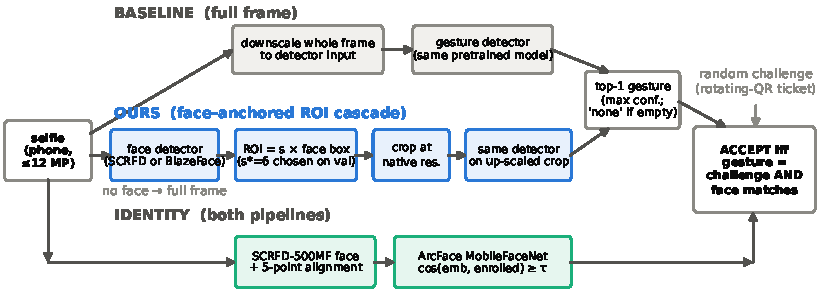
\includegraphics[width=0.92\linewidth]{figures/pipeline.pdf}
  \vspace{-2mm}
  \caption{\textbf{Pipeline.} Baseline (top): the gesture detector sees the whole, downscaled frame. Ours
  (middle): face detector $\rightarrow$ ROI $=s\times$ face box $\rightarrow$ the same detector on the crop. The
  detections are mapped back to image coordinates. Both pipelines share the identity branch (bottom) and the
  accept rule.}
  \label{fig:pipeline}
  \vspace{-3mm}
\end{figure*}

\noindent\textbf{Baseline.} The gesture detector runs on the full image. The predicted gesture is the class of
the highest-confidence detection, or \texttt{none} if there is no detection.

\noindent\textbf{Proposed cascade} (\cref{fig:pipeline}). (1)~A face detector finds faces, and the \emph{largest}
one is taken as the selfie-taker. The proposal used BlazeFace short-range (MediaPipe Tasks, conf.\ 0.5). We also
test SCRFD-500MF, which the identity branch runs anyway. (2)~The ROI is a box of $s\cdot w_f\times s\cdot h_f$
centred on the face, clipped to the image and rounded to whole pixels. The proposal fixed $s{=}3$; the final
system uses the anchor and $s$ chosen on the val split (\cref{sec:exp}). (3)~The crop is passed to the detector at
native resolution, so the detector's own resizing \emph{up-scales} small crops. (4)~Detections are shifted back by
the crop offset, and the top-1 rule is the same as the baseline's. If no face is found, the pipeline falls back to
the full frame. This fallback is counted and reported.

\noindent\textbf{Gesture detector.} Both pipelines use Google's \emph{pretrained} MediaPipe Gesture
Recognizer~\cite{mphands} (palm detector, 21 hand landmarks, gesture classifier), the same model the deployed app
uses. Its classes are mapped to five HaGRID gestures (like, peace, palm, fist, one; it has no ``ok''). We keep a
label only if its score is $\geq$0.5, and its box is the landmark extent. The detector was trained by a third
party, so neither pipeline has seen our data. The detector is an interchangeable module: the repository also
contains a YOLOv8n~\cite{yolov8} fine-tuning path (\texttt{train\_yolo.py}), which we did not evaluate for this
report.

\noindent\textbf{Identity.} SCRFD-500MF~\cite{scrfd} detects the face and its 5 landmarks. The face is aligned to
112$\times$112 and embedded by ArcFace MobileFaceNet~\cite{mobilefacenet,arcface} (InsightFace \texttt{buffalo\_s},
run with onnxruntime). A probe is accepted when its cosine similarity to the enrolled embedding is $\geq\tau$.
$\tau{=}\lfwThr$ maximises accuracy on LFW~\cite{lfw} DevTrain (DevTest: \lfwTestAcc\% accuracy, FAR
\lfwTestFAR\%, FRR \lfwTestFRR\%), with no training on our data.

%% ------------------------------------------------------------------------------------------- Dataset
\section{Dataset}
\label{sec:data}

\noindent\textbf{Source and labels.} HaGRIDv2~\cite{hagridv2} (CC BY-SA 4.0 variant) has 1.08M FullHD images of
consenting subjects. Each image has gesture boxes and labels, a \texttt{user\_id}, and \emph{automatically
estimated} age, gender and race. We use HaGRID's \emph{official subject-disjoint} split and the gesture classes
like, peace, palm, fist, ok and one. MediaPipe is scored on the 5 of them it supports. The archives are 40\,GB per
class, so \texttt{fetch\_hagrid.py} reads the ZIP central directories with HTTP range requests and downloads only
the selected images ($\approx$1.2\,GB, 2\,min).

\noindent\textbf{Split and size.} \emph{Test}: 603 test subjects show all six gestures. We draw 100 of them at
random (seed 441) and take one image per (subject, gesture). This gives \textbf{600 images at native resolution}
(mostly 1440$\times$1920; 60\% of images female, 80\% annotated White). \emph{Val}: 50 images per class, each from
a different val subject (300). The val set is used only to choose the ROI settings. The image ids are stored in
\texttt{selection.json}. No test subject appears in val.

\noindent\textbf{Test conditions (our construction).}
The proposal planned a volunteer set captured in a classroom, which we did not collect (\cref{sec:fail}).
Instead, \texttt{make\_conditions.py} derives four conditions from each source image. Each output is a
deterministic function of (image, condition, seed), so the baseline and ours see identical inputs (\cref{fig:cond}).
\emph{normal}: unchanged.
\emph{low light}: brightness $\times$0.35, gamma 1.4, Gaussian noise $\sigma{=}6$, JPEG q85.
\emph{far}: the image is pasted at native resolution into the centre of a canvas twice as wide and twice as tall, so the subject covers $\frac{1}{4}$ of the frame.
\emph{crowded}: a \emph{different} subject showing a \emph{different} gesture is pasted at 0.6$\times$ scale
beside the claimant. This doubles as the \emph{background-hand attack}: if the challenge is the other person's
gesture, a correct system must reject.
The result is 2,400 test images (2,000 with MediaPipe's 5 gestures) and, from the val images, a 1,200-image val set.

\begin{figure}[t]
  \centering
  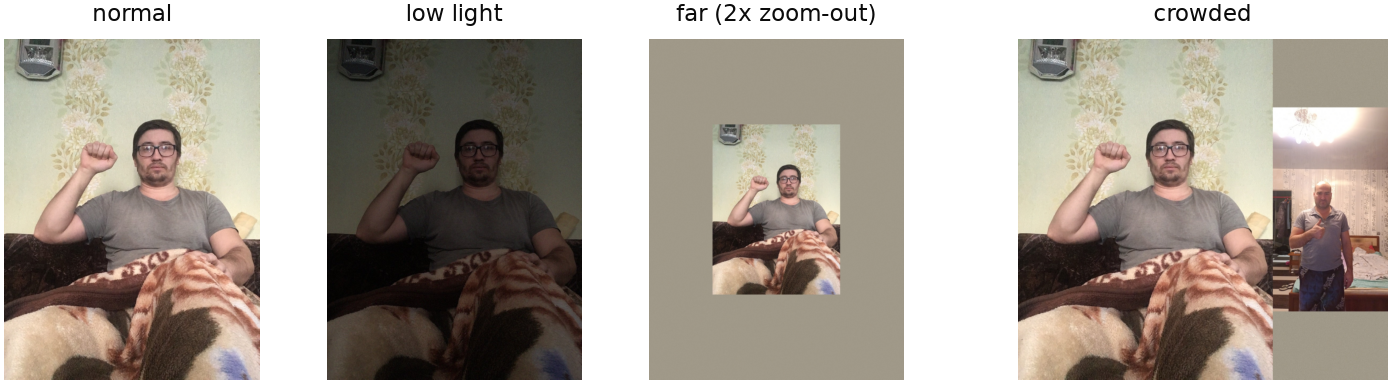
\includegraphics[width=\linewidth]{figures/conditions.png}
  \vspace{-1.5mm}
  \caption{One held-out subject in the four test conditions (crowded: another test subject added at 0.6$\times$).}
  \label{fig:cond}
  \vspace{-3mm}
\end{figure}

%% ------------------------------------------------------------------------------------------- Experiments
\section{Experiments}
\label{sec:exp}

\noindent\textbf{Protocol.} Every configuration runs on the same 2,400 test images with the same pretrained
detector. Face detection runs once per image and is shared by all ROI variants of that anchor
(\texttt{predict.py}), so only the ROI geometry and the anchor change. The face threshold comes from LFW and the ROI
settings come from the val set, never from test.
\emph{Model selection}: the proposal fixed $s{=}3$ with BlazeFace, and we test that setting as pre-registered.
We also choose the anchor and scale on the 1,200-image val set, built the same way from other subjects. The grid
is \{BlazeFace, SCRFD\} $\times$ $s\in\{2,\dots,6\}$, ties go to BlazeFace and then to the smaller $s$, and the
selected setting is evaluated on test once.

\noindent\textbf{Metrics.} \emph{Quality}: top-1 gesture accuracy (the decision the app makes), with 95\%
bootstrap CIs~\cite{efron}. \emph{Comparison}: the paired accuracy change, with a paired-bootstrap 95\% CI and an
exact McNemar test~\cite{mcnemar} on the discordant images. \emph{Security}: background-hand FAR (crowded images,
challenge = the other person's gesture) and end-to-end FRR/FAR with ArcFace. Each subject's first normal image is
the enrollment; the other 23 images are probes. \emph{Cost}: median and p95 CPU latency per selfie, detector calls
and model size. H1 holds if the overall gain is $\geq$5\,pp with a CI that excludes 0, and the extra median latency
is $\leq$50\,ms.

%% ------------------------------------------------------------------------------------------- Results
\section{Results}
\label{sec:results}

\begin{table*}[t]
\centering
\small
\setlength{\tabcolsep}{6pt}
\begin{tabular}{lccccc}
\toprule
Pipeline & Normal & Low light & Far (2$\times$) & Crowded & All \\
\midrule
Baseline (full frame) & 91.0 & 67.0 & 63.6 & 70.0 & 72.9 \\
Ours, $s{=}3$ (proposal) & 67.8 {\scriptsize($-$23.2$^\dagger$)} & 47.2 {\scriptsize($-$19.8$^\dagger$)} & 64.6 {\scriptsize(+1.0)} & 66.8 {\scriptsize($-$3.2)} & 61.6 {\scriptsize($-$11.3$^\dagger$)} \\
Ours, $s^*{=}6$, SCRFD (val-sel.) & 93.8 {\scriptsize(+2.8$^\dagger$)} & 77.0 {\scriptsize(+10.0$^\dagger$)} & 94.0 {\scriptsize(+30.4$^\dagger$)} & 77.4 {\scriptsize(+7.4$^\dagger$)} & 85.5 {\scriptsize(+12.7$^\dagger$)} \\
\bottomrule
\end{tabular}
\vspace{-1mm}
\caption{\textbf{Main comparison} on the 100 held-out HaGRID subjects. Top-1 gesture accuracy (\%), with the paired change vs.\ the baseline in pp; $^\dagger$: exact McNemar $p<0.05$. Both pipelines use the \emph{same} pretrained MediaPipe Gesture Recognizer, scored on its 5 classes (2,000 images, 500 per condition). 95\% bootstrap CIs of the overall change are given in the text.}
\label{tab:main}
\vspace{-2mm}
\end{table*}

\noindent\textbf{Main comparison} (\cref{tab:main}). The \emph{pre-registered} cascade ($s{=}3$, BlazeFace)
is worse than the baseline: \mpSAllD\,pp overall (95\% CI [\mpSAllLo, \mpSAllHi]) and \mpSNorD\,pp on normal
images. It breaks \mpSAllBrk{} images and fixes only \mpSAllFix. With this setting \textbf{H1 is rejected}. The
setting \emph{selected on val} ($s^*{=}\mpTScale$, SCRFD anchor; val accuracy \mpValSSixscrfd\% vs.\
\mpValfull\% for the full frame) raises test accuracy from \mpBaseAllAcc\% to \mpTAllAcc\%, a gain of
\mpTAllD\,pp (CI [\mpTAllLo, \mpTAllHi], McNemar $p\mpTAllP$; \mpTAllFix{} fixed vs.\ \mpTAllBrk{} broken). It
improves every condition: \mpTFarD\,pp far, \mpTLowD\,pp low light, \mpTCroD\,pp crowded, and \mpTNorD\,pp normal
($p{=}\mpTNorP$). The gain comes from where the hand is small or degraded, as hypothesised, and the extra median
latency is \latExtramediapipe\,ms (\cref{tab:cost}). With the val-selected setting, \textbf{H1 is supported}.
Note, however, that this is not the setting we fixed in advance.

\begin{table}[t]
\centering
\footnotesize
\setlength{\tabcolsep}{2.6pt}
\begin{tabular}{lcccc}
\toprule
 & \multicolumn{4}{c}{MediaPipe} \\
\cmidrule(lr){2-5}
 & \multicolumn{2}{c}{BlazeFace} & \multicolumn{2}{c}{SCRFD} \\
$s$ & all & far & all & far \\
\midrule
full frame & \multicolumn{4}{c}{72.9 / 63.6} \\
\midrule
2 & 41.1 & 63.2 & 2.5 & 3.0 \\
3 (prop.) & 61.6 & 64.6 & 26.1 & 29.4 \\
4 & 73.1 & 64.4 & 66.0 & 72.6 \\
5 & 74.6 & 64.2 & 83.1 & 90.6 \\
6 & 74.6 & 64.2 & \textbf{85.5} & \textbf{94.0} \\
\midrule
3, no up-scale & 62.8 & 64.8 &  &  \\
3, shift $0.5h_f$ & 62.2 & 64.6 &  &  \\
\midrule
face found & 71.2 & 13.7 & 99.7 & 99.0 \\
\bottomrule
\end{tabular}
\vspace{-1mm}
\caption{\textbf{Ablation}: top-1 accuracy (\%) on all 4 conditions / far only, by ROI scale $s$ and face anchor; every cell uses the same detector weights and images. Bold: the configuration selected on the val split. ``face found'': \% of normal / far images in which the anchor found a face (otherwise the pipeline falls back to the full frame).}
\label{tab:abl}
\vspace{-3mm}
\end{table}

\noindent\textbf{Ablation} (\cref{tab:abl}). \emph{ROI size} matters most. HaGRID subjects hold the hand beside
the head, often more than one face-width away, so $s{\le}3$ cuts it off and accuracy falls far below the
baseline. It rises up to $s{=}6$, the edge of our grid, so a larger $s$ could be better still.
The \emph{anchor} decides the far condition. BlazeFace short-range finds a face in only \mpFaceSThreeUpnormal\% of
normal and \mpFaceSThreeUpfar\% of far images, and otherwise falls back to the full frame, so BlazeFace ROIs
cannot beat the baseline on far images. SCRFD finds a face in $\geq$98\% of the images in every condition.
SCRFD boxes are tighter, so SCRFD needs $s{\ge}5$, but at that size it lifts far accuracy to
\mpAccFarSSixUpScrfd\%.
\emph{Up-scaling} and \emph{shifting the ROI} down by half a face change accuracy by ${\approx}1$\,pp at $s{=}3$.

\begin{table}[t]
\centering
\footnotesize
\setlength{\tabcolsep}{4pt}
\begin{tabular}{lccc}
\toprule
Pipeline & median & p95 & extra \\
\midrule
full frame & 15.6 & 22.2 & -- \\
ROI $s{=}3$, BlazeFace & 17.4 & 24.3 & +1.8 \\
ROI $s{=}6$, SCRFD & 22.1 & 28.7 & +6.4 \\
\midrule
SCRFD + ArcFace (both) & 10.0 & 18.9 & -- \\
\bottomrule
\end{tabular}
\vspace{-1mm}
\caption{\textbf{Cost}: CPU latency per selfie in ms (100 native-resolution test images, cpu, Ryzen 7 7800X3D, decode excluded). The ROI pipeline includes the anchor face detector and the crop, and makes one face-detector call plus one gesture-detector call per image. Model sizes: MediaPipe GR 8.0\,MB, BlazeFace 0.22\,MB, SCRFD 2.4\,MB, ArcFace 13.0\,MB.}
\label{tab:cost}
\vspace{-3mm}
\end{table}
\begin{table}[t]
\centering
\footnotesize
\setlength{\tabcolsep}{2.2pt}
\begin{tabular}{lccccc}
\toprule
Pipeline & FRR & FAR$_\text{bg}$ & FAR$_\text{face}$ & FAR$_\text{gest}$ & FAR$_\text{rep}$ \\
\midrule
full & 30.1 & 13.6 & 0.65 & 0.95 & 45.2 \\
ROI $s{=}3$, BlazeFace & 40.4 & 7.1 & 0.58 & 0.70 & 36.7 \\
ROI $s{=}6$, SCRFD & 15.3 & 0.8 & 0.75 & 0.21 & 46.5 \\
\bottomrule
\end{tabular}
\vspace{-1mm}
\caption{\textbf{End-to-end} accept/reject (\%; gesture \emph{and} ArcFace, $\tau{=}0.2235$). FRR: genuine check-ins rejected (all conditions). FAR$_\text{bg}$: the challenge is the gesture of the \emph{other} person in a crowded image. FAR$_\text{face}$: another enrolled student's identity is claimed. FAR$_\text{gest}$: a wrong gesture is accepted. FAR$_\text{rep}$: an old photo passes a random challenge within 3 attempts.}
\label{tab:sec}
\vspace{-3mm}
\end{table}

\noindent\textbf{Cost} (\cref{tab:cost}). Both pipelines make one gesture-detector call. The cascade adds one
face-detector call and a crop. With SCRFD the face detection can be shared with the identity branch, which runs
SCRFD anyway, so in a deployed system the added cost is close to zero.

\noindent\textbf{End to end} (\cref{tab:sec}). With face verification included, the val-selected cascade halves
the false-reject rate (\mpFRRFull\%$\rightarrow$\mpFRRRoiSix\%; far: \mpFRRFullfar\%$\rightarrow$\mpFRRRoiSixfar\%).
It also blocks the background-hand attack (\mpFARbgFull\%$\rightarrow$\mpFARbgRoiSix\%). With the ROI, the gesture
and the verified face come from the same person: an attacker who copies a classmate's gesture is matched against
the face next to that hand, and that face is not theirs. Impostor-face FAR stays below 1\%. On LFW-calibrated
ArcFace, normal images give FRR \faceFRRnormal\% and FAR \faceFARnormal\%.

\begin{figure*}[t]
  \centering
  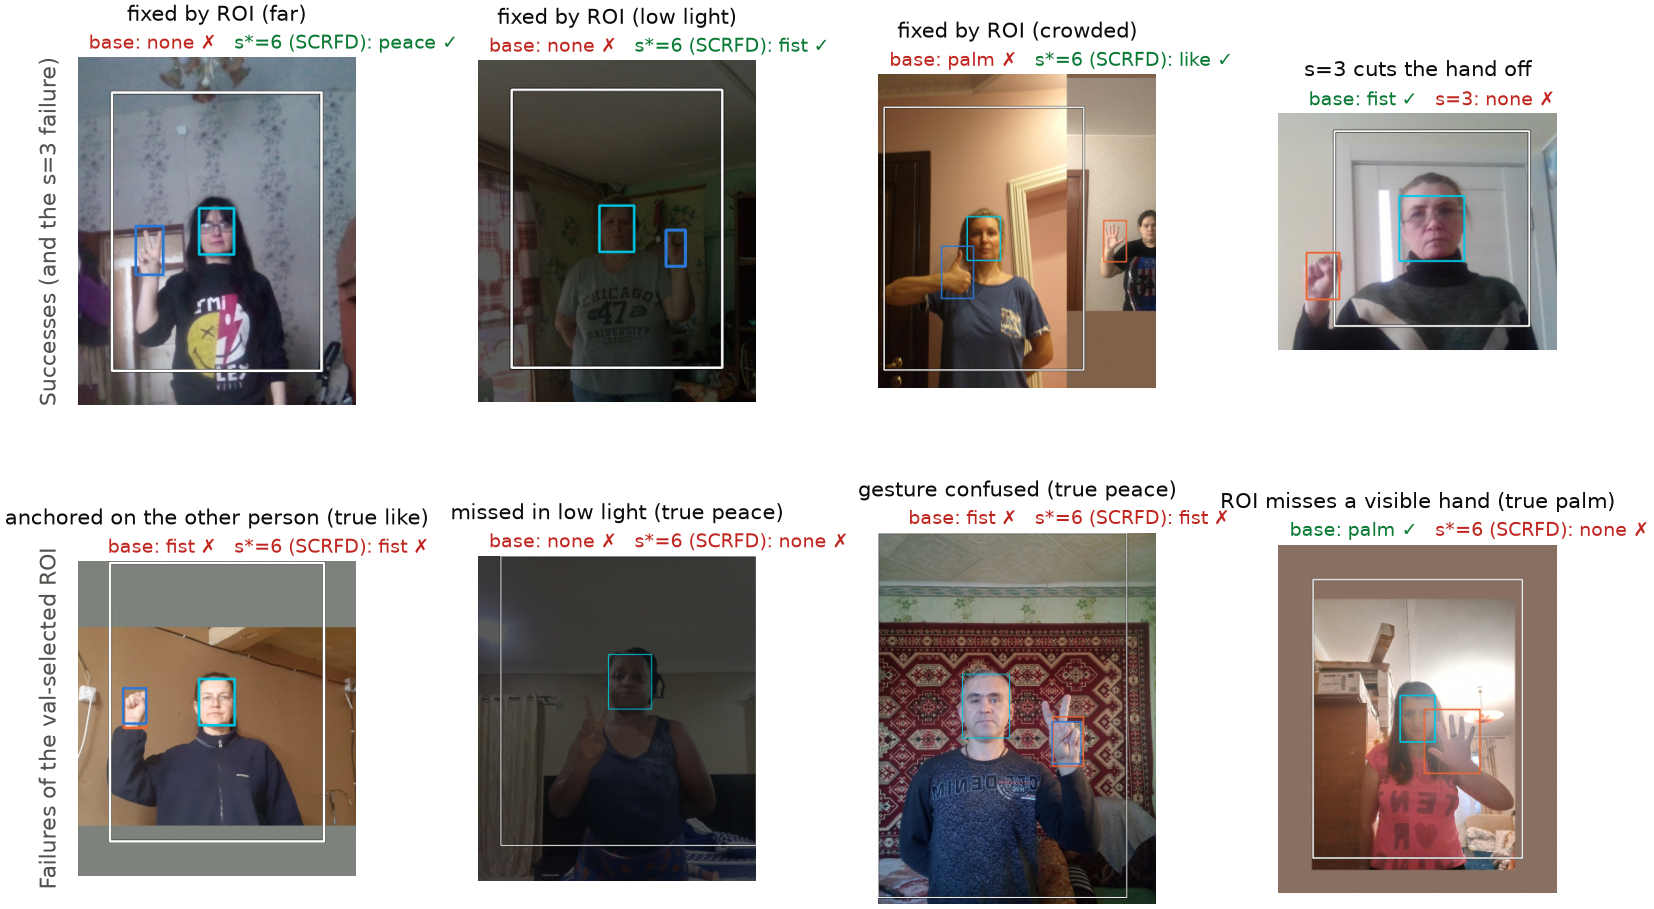
\includegraphics[width=0.8\linewidth]{figures/qualitative.png}
  \vspace{-1.5mm}
  \caption{\textbf{Qualitative examples} (held-out test images, zoomed). White: ROI; cyan: anchor face;
  orange: baseline's top detection; blue: ours. Top: successes of the val-selected ROI and the typical failure of
  the proposal's $s{=}3$. Bottom: failures of the val-selected ROI.}
  \label{fig:qual}
  \vspace{-3mm}
\end{figure*}

%% ------------------------------------------------------------------------------------------- Failures
\section{Failure analysis and limitations}
\label{sec:fail}

\noindent\textbf{Where it fails} (\cref{fig:qual}, bottom). Of the \mpTErrErrors{} errors of the val-selected
cascade, \mpTErrNoDetectionInRoi{} are hands that MediaPipe misses inside the ROI. These are mostly in low light
(\mpTErrErrorsLowLight{} errors) and in crowded images (\mpTErrErrorsCrowded). \mpTErrWrongClass{} are wrong
classes and only \mpTErrNoFaceFound{} have no face. \mpTErrBaselineAlsoWrong{} of the \mpTErrErrors{} errors are also
made by the baseline. (1)~\emph{Wrong anchor}: the ``largest face'' rule picks the background person in
\mpWrongAnchorSSixUpScrfd\% of crowded images, because that person's face can be bigger in pixels. The genuine
student is then rejected; the attack still fails, since the face does not match. (2)~\emph{ROI too small}: the
proposal's $s{=}3$ cuts off hands held at arm's length (top right). The ROI size is a property of how users pose,
so it must be validated on the target population. (3)~\emph{Replay}: a stored photo passes a random 1-of-5
challenge within 3 attempts 36.7--46.5\% of the time, whichever pipeline is used. The gesture challenge alone is weak liveness;
two-gesture challenges or fewer attempts are needed.

\noindent\textbf{Bias.} On HaGRID's automatic labels (aggregated per subject), the val-selected cascade scores
\mpBiasTgenderfemale\% for female and \mpBiasTgendermale\% for male subjects, and \mpBiasTagegroupYoung\% for
subjects under 25 vs.\ \mpBiasTagegroupOld\% for those over 40. This narrows the baseline's age gap
(\mpBiasFullagegroupYoung\% vs.\ \mpBiasFullagegroupOld\%). Only \mpBiasNraceBlack{} Black, \mpBiasNraceAsian{} Asian
and \mpBiasNraceIndian{} Indian subjects are in the test set, too few for conclusions about race. Face verification
bias was not measured per group.

\noindent\textbf{Limitations.} The far, low-light and crowded conditions are \emph{synthetic}: real distance also
blurs the image and real low light changes the noise. We did not collect the planned classroom volunteer set, so
there are no real phone selfies from our own population; this is the most important missing evidence. HaGRID
subjects are 80\% White. The tested scales stop at the grid edge. Only one gesture detector was evaluated.
InsightFace weights are licensed for non-commercial research only, and storing face embeddings needs consent and a
deletion policy. The app keeps only embeddings and lets the instructor delete them.

%% ------------------------------------------------------------------------------------------- Implementation
\section{Implementation and attribution}
\label{sec:impl}

\noindent\textbf{Built by the team:} the ROI cascade (ROI geometry, crop/up-scale, coordinate mapping, fallback)
and the controlled baseline; the attendance web app (3\,s rotating QR tokens, phone-bound tickets, random
challenge, enrollment with instructor confirmation, flags, Excel reports); the HaGRID range-request fetcher, the
four-condition test set and attack construction; all evaluation, statistics, latency and figure scripts; and the
fine-tuned YOLOv8n weights.
\textbf{External:} Ultralytics YOLOv8 code and COCO \texttt{yolov8n.pt} (AGPL-3.0); MediaPipe Gesture
Recognizer and BlazeFace (Apache-2.0); InsightFace \texttt{buffalo\_s} SCRFD/ArcFace weights (non-commercial
research); HaGRIDv2 images and annotations; LFW (threshold only); the CVPR author kit.
\textbf{Generative AI:} an AI coding assistant (Claude, via Claude Code) wrote most of the code and first drafts
of this report and the slides, under the team's direction. All numbers come from the released scripts; none
was typed in by hand.
Code, split and a one-command reproduction (\texttt{reproduce.ps1}, $\approx$2.5\,h on a CPU) are submitted.


{
\small
\bibliographystyle{ieeenat_fullname}
\bibliography{refs}
}

\end{document}
